\chapter{Architectural Overview}
\label{ch:architectural_overview}
In this chapter, the architectural overview of the run-time state migration approach is discussed. First, the publish-subscribe pattern is explained as a mean to exchange state information and manage available devices as well as which state models are supported by an application. The middleware is explained next, which uses the publish-subscribe pattern and acts as a message broker. Subsequently, the library as well as the interfaces that need to be implemented by the respective applications are explained. Moreover, we explain the message exchange in the different life cycle phases of the migration approach. The last part explains the Model Repository and suggests an improved concept.

\section{Publish–subscribe pattern}
An infrastructure is needed to exchange run-time states of applications across different devices. Also, devices should know which other devices with common Application State Models are available and notice if they join or leave the network. Moreover, devices should be able to migrate the run-time state and acknowledge other devices when migration is done.

In this approach, we chose to use the publish-subscribe pattern. Thereby, the middleware is the message broker, devices are publishers and subscribers, Application State Models are topics, and run-time states are messages. Also, there are extra topics and messages that allow us to fulfil requirements such as device introduction, device connectivity and finalizing the run-time state migration.

Figure \ref{fig:publish–subscribe} illustrates an overview of publish–subscribe pattern in our approach. A Mac device (see \fcircone) subscribes to \textit{Model-A} and \textit{Model-B} topics, a Windows device (see \fcirctwo) subscribes to \textit{Model-A} topic and an Android device (see \fcircthree) subscribes to \textit{Model-B} topic. The Mac device publishes a message contain \textit{"X"} to topic \textit{Model-A}, and the middleware makes sure it gets forwarded to the Windows device. Also, a message containing \textit{"Y"} is published from the Mac device to the topic \textit{Model-B} and forwarded to the Android device by the middleware.

\vspace{10mm}
\FloatBarrier \begin{figure}[H]
    \includegraphics[width=0.8\textwidth]{../figures/publish-subscribe.pdf}
    \centering
    \caption{Overview of Publish–subscribe pattern in our approach.}
    \label{fig:publish–subscribe}
\end{figure} \FloatBarrier

\subsection{Middleware}
As the middleware acts as a message broker, if devices are not on the same network, a middleware should exist in which applications can communicate with each other. Figure \ref{fig:solution-overview} shows the role of middleware.
This middleware can handle sending and receiving the run-time state.
The goal of having this middleware is applications which coupled with
libraries, can introduce themselves, find each other, and migrate the run-time state.

Also, as mentioned in \textbf{R4 Device Management}, the middleware is responsible for device discovery and notifying other devices if a device joins or leaves with the same Application State Model. The message exchange for device discovery is explains in subchapter 6.5.

As in this thesis, we considered the publish-subscribe pattern as the architecture, the middleware is the intermediary message broker.

\subsection{Topics}
There are some topics each device should subscribe to them. Devices who subscribed to these topics receive a message if another device publish a message to them.

\subsubsection{Topic for Connectivity Status}
All devices should subscribe to a topic about their connectivity status. This topic is \lstinline[basicstyle=\ttfamily]{online}. If a device joins or leaves the network, other devices get notice by a message.

\subsubsection{Topics for Application State Models}
Each Application State Model has a topic. Devices that supports these Application State Models should subscribe to these topics. So, if a device joins the same topic, it should notify other devices about joining and supporting the same Application State Model and also other devices notify the new device about their existence as a response. Moreover, for each Application State Model, devices should subscribe to the subtopic of device identification, that they can receive an individual message from other devices and vice versa. As users may use different devices and applications device identification must be unique like UUID; to improve the readability of the following example, we use a combination of the operating system and application name as the UUID. Of course, the is only done for the examples in the thesis and would lead to name clashes in a broader scenario. In a live setting, the UUID would be randomly generated.



\subsubsection{Example Scenario}
Considering the scenario of Figure \ref{fig:asml-overview}. Three devices share some Application State Models. All devices should subscribe to \lstinline[basicstyle=\ttfamily]{online} topic. Mailspring supports three Application State Models, so it should subscribe to topics:
\begin{verbatim}
online
search
new-event
sending-email
\end{verbatim}

Also, to guarantee that other devices on the same topic can send message to Mailspring, it should subscribe to these subtopics with its identification: 
\begin{verbatim}
search/mac-mailspring
new-event/mac-mailspring
sending-email/mac-mailspring
\end{verbatim}

As K-9 Mail supports two Application State Models, it has to subscribe to these topics:
\begin{verbatim}
online
search
sending-email
search/android-k9mail
sending-email/android-k9mail
\end{verbatim}


Also, as Woven supporting one Application State Model, it has to subscribe to these topics:
\begin{verbatim}
online
new-event
new-event/windows-woven
\end{verbatim}

% So, if K-9 Mail and Woven are already in the network and Mailspring joins, it  sends a message to topics \lstinline[basicstyle=\ttfamily]{search}, \lstinline[basicstyle=\ttfamily]{sending-email} and \lstinline[basicstyle=\ttfamily]{new-event} which allows K-9 Mail and Woven get notify about joining the new device with common Application State Models. Also, Woven sends back a introduction response message to \lstinline[basicstyle=\ttfamily]{new-event/mac-mailspring} about its existence. Morever, K-9 Mail should do the same but to \lstinline[basicstyle=\ttfamily]{search/mac-mailspring} and \lstinline[basicstyle=\ttfamily]{sending-email/mac-mailspring} topics.


\subsection{Messages}
In this architecture, we need some message to fulfill our requirements like device introduction and transferring a run-time state.

\subsubsection{Device Introduction}
When a user runs an application, the application should introduce itself to other devices on the network. Moreover, other devices should get notify and response about their existence by an introduction.

\subsubsection{Device Leave}
After an application got closed or a device went offline, it should notify other devices about its absence. Moreover, other devices should not be able to communicate with that device anymore.

\subsubsection{Device Has Run-time State}
If a device has a run-time state, it should notify other devices which support  common Application State Model about having a run-time state.

\subsubsection{Request Run-time State}
A device can request a run-time state of other devices supporting the common Application State Model. The source device should respond to this request by sending its run-time state.

\subsubsection{Send Run-time State}
As the target device can request a run-time state, the source device should respond to this request by sending its run-time state. Also, the target application should be aware of receiving it.

\subsubsection{Finalizing Run-time State Migration}
After the target device received a run-time state and is adjusted into the application, the target device should notify the source device about finalizing the run-time state migration to react to this message like by resetting its UI and removing its run-time state.

\subsection{Actions}
In this architecture, we need some actions to fulfill our requirements, like store a run-time state and adding the new device that joined recently.

\subsubsection{Store Run-time State}
When a device has a run-time state, it should be stored in case other devices request a run-time state migration.

\subsubsection{Add Device}
Whenever a device receives a Device Introduction message, it should add the device to its list so that it can access it in the future.

\subsubsection{Remove Device}
Whenever a device receives a Device Leave message, it should remove that particular device from its list to prevent further communication.

\section{Library}
As state in \textbf{R1 Applicable on Existing Applications}, this approach is meant to support run-time state migration for existing applications on different platforms; special libraries in different programming languages and platforms should be developed. 
These libraries should provide basic functionality such as communication, validation of run-time states based on an Application State Model, and an API to support extraction and injection of run-time states between same-purpose applications with common Application State Model.

Developers can integrate these libraries in existing applications to enable run-time state migration, and they should implement some glue code in existing source code to adapt the library into existing applications (Figure \ref{fig:solution-overview}). The library reflect are the generic part of run-time state migration, the glue code and the interfaces derived from the application state model reflect the application specific part.

These libraries should be written in the same programming languages as the source and target applications. They should be able to communicate directly or with the help of the middleware.
If devices are on the same local network, these libraries should establish a point-to-point connection.
Otherwise, they should be able to communicate with help the middleware over the internet.
In this case, they should introduce themselves to the middleware to find each other; then, they can migrate the run-time state. As mentioned before, the focus of the thesis is not providing different types of communications, only indirect communication with help of the middleware should be implemented.


\section{Interfaces}
Interfaces are derived from Application State Model, and they guarantee certain values on a run-time state. They can be auto-generated or manually written by developers with same programming language of the source and target applications.
To integrate the libraries into source code, developers should implement some glue code and use the interfaces like Figure \ref{fig:solution-overview}. Developers should add interfaces to the library with glue code. Thereby, the library will know which Application State Models has to be supported.

Considering Mailspring written in TypeScript, Listing \ref{lis:search-interface} shows a generated interface based on search Application State Model (Listing \ref{lis:search-schema}).

\FloatBarrier
\begin{code}
\begin{js}
export interface SearchObject {
    /**
     * the query of search
     */
    query: string;
    /**
     * shows if the query is already has been submitted
     */
    submit?: boolean;
}
\end{js}
\caption{Search example interface in TypeScript.}
\label{lis:search-interface}
\end{code}
\FloatBarrier


\section{Life Cycles}
After explanation of entities of the architecture in previous sections, the interaction between these entities in different life cycle phases is explained. These life cycles phases consist of main entities, actions and sequence of messages discussed in the messages section, and they are implemented in chapter \ref{ch:implementation}. 
\subsection{Initializing}
\begin{figure}
    \includegraphics[width=\linewidth]{../figures/Initializing-Mailspring}
    \centering
    \caption{Initializing: Mailspring}
    \label{fig:Initializing-Mailspring}
\end{figure}

\subsection{Run-time State Management}
\subsubsection{Store State}
\begin{figure}
    \includegraphics[width=\linewidth]{../figures/Store-Current-State}
    \centering
    \caption{Store the Current State}
    \label{fig:Store-Current-State}
\end{figure}
\subsubsection{Has State}
\begin{figure}
    \includegraphics[width=\linewidth]{../figures/Inform-Devices-Has-State-Mailspring}
    \centering
    \caption{Inform other devices has a State: Mailspring}
    \label{fig:Inform-Devices-Has-State-Mailspring}
\end{figure}

\subsection{Migration Patterns}
\subsubsection{Pull Method}
\begin{figure}
    \includegraphics[width=\linewidth]{../figures/Migration-Mailspring-to-K9-Pull-Method}
    \centering
    \caption{Pull Method: Migration Mailspring to K9}
    \label{fig:Migration-Mailspring-to-K9-Pull-Method}
\end{figure}

\subsubsection{Push Method}
\begin{figure}
    \includegraphics[width=\linewidth]{../figures/Migration-Mailspring-to-K9-Push-Method}
    \centering
    \caption{Push Method: Migration Mailspring to K9}
    \label{fig:Migration-Mailspring-to-K9-Push-Method}
\end{figure}

\subsection{Going Offline}
\subsubsection{Graceful}
\begin{figure}
    \includegraphics[width=\linewidth]{../figures/Going-Offline-Graceful-Mailspring}
    \centering
    \caption{Going Offline Gracefully: Mailspring}
    \label{fig:Going-Offline-Graceful-Mailspring}
\end{figure}
\subsubsection{Ungraceful}
\begin{figure}
    \includegraphics[width=\linewidth]{../figures/Going-Offline-Ungraceful-Mailspring}
    \centering
    \caption{Going Offline Ungracefully: Mailspring}
    \label{fig:Going-Offline-Ungraceful-Mailspring}
\end{figure}


\section{Model Repository}

As stated in requirement \textbf{R3 Model Repository}, we made a repository manager call Model Repository located on GitHub\footnote{\url{https://github.com/asml-lang/model-repository}}. Some models are available on this repository. Developers may use the search ability of GitHub to find their suitable Application State Models. Also, after making a new model, developers can add it the repository manager by making a pull request. So, other developers may use it for their applications.

Currently, a GitHub repository is sufficient for this thesis. Although conceptually, we may be able to improve the Model Repository so that developers may easily search the model they need by name, description, or keywords and download or customize them. In addition, if the developer does not find the model they need, they could create a custom model using the Model Repository editor. Additionally, if they have already developed a model, they may upload it to the Model Repository. The concept behind the solution is valid; however, implementation is a future work objective. Figure \ref{fig:model-repo} is an improved Model Repository that shown as a wireframe concept.

\FloatBarrier
\begin{figure}[H]
    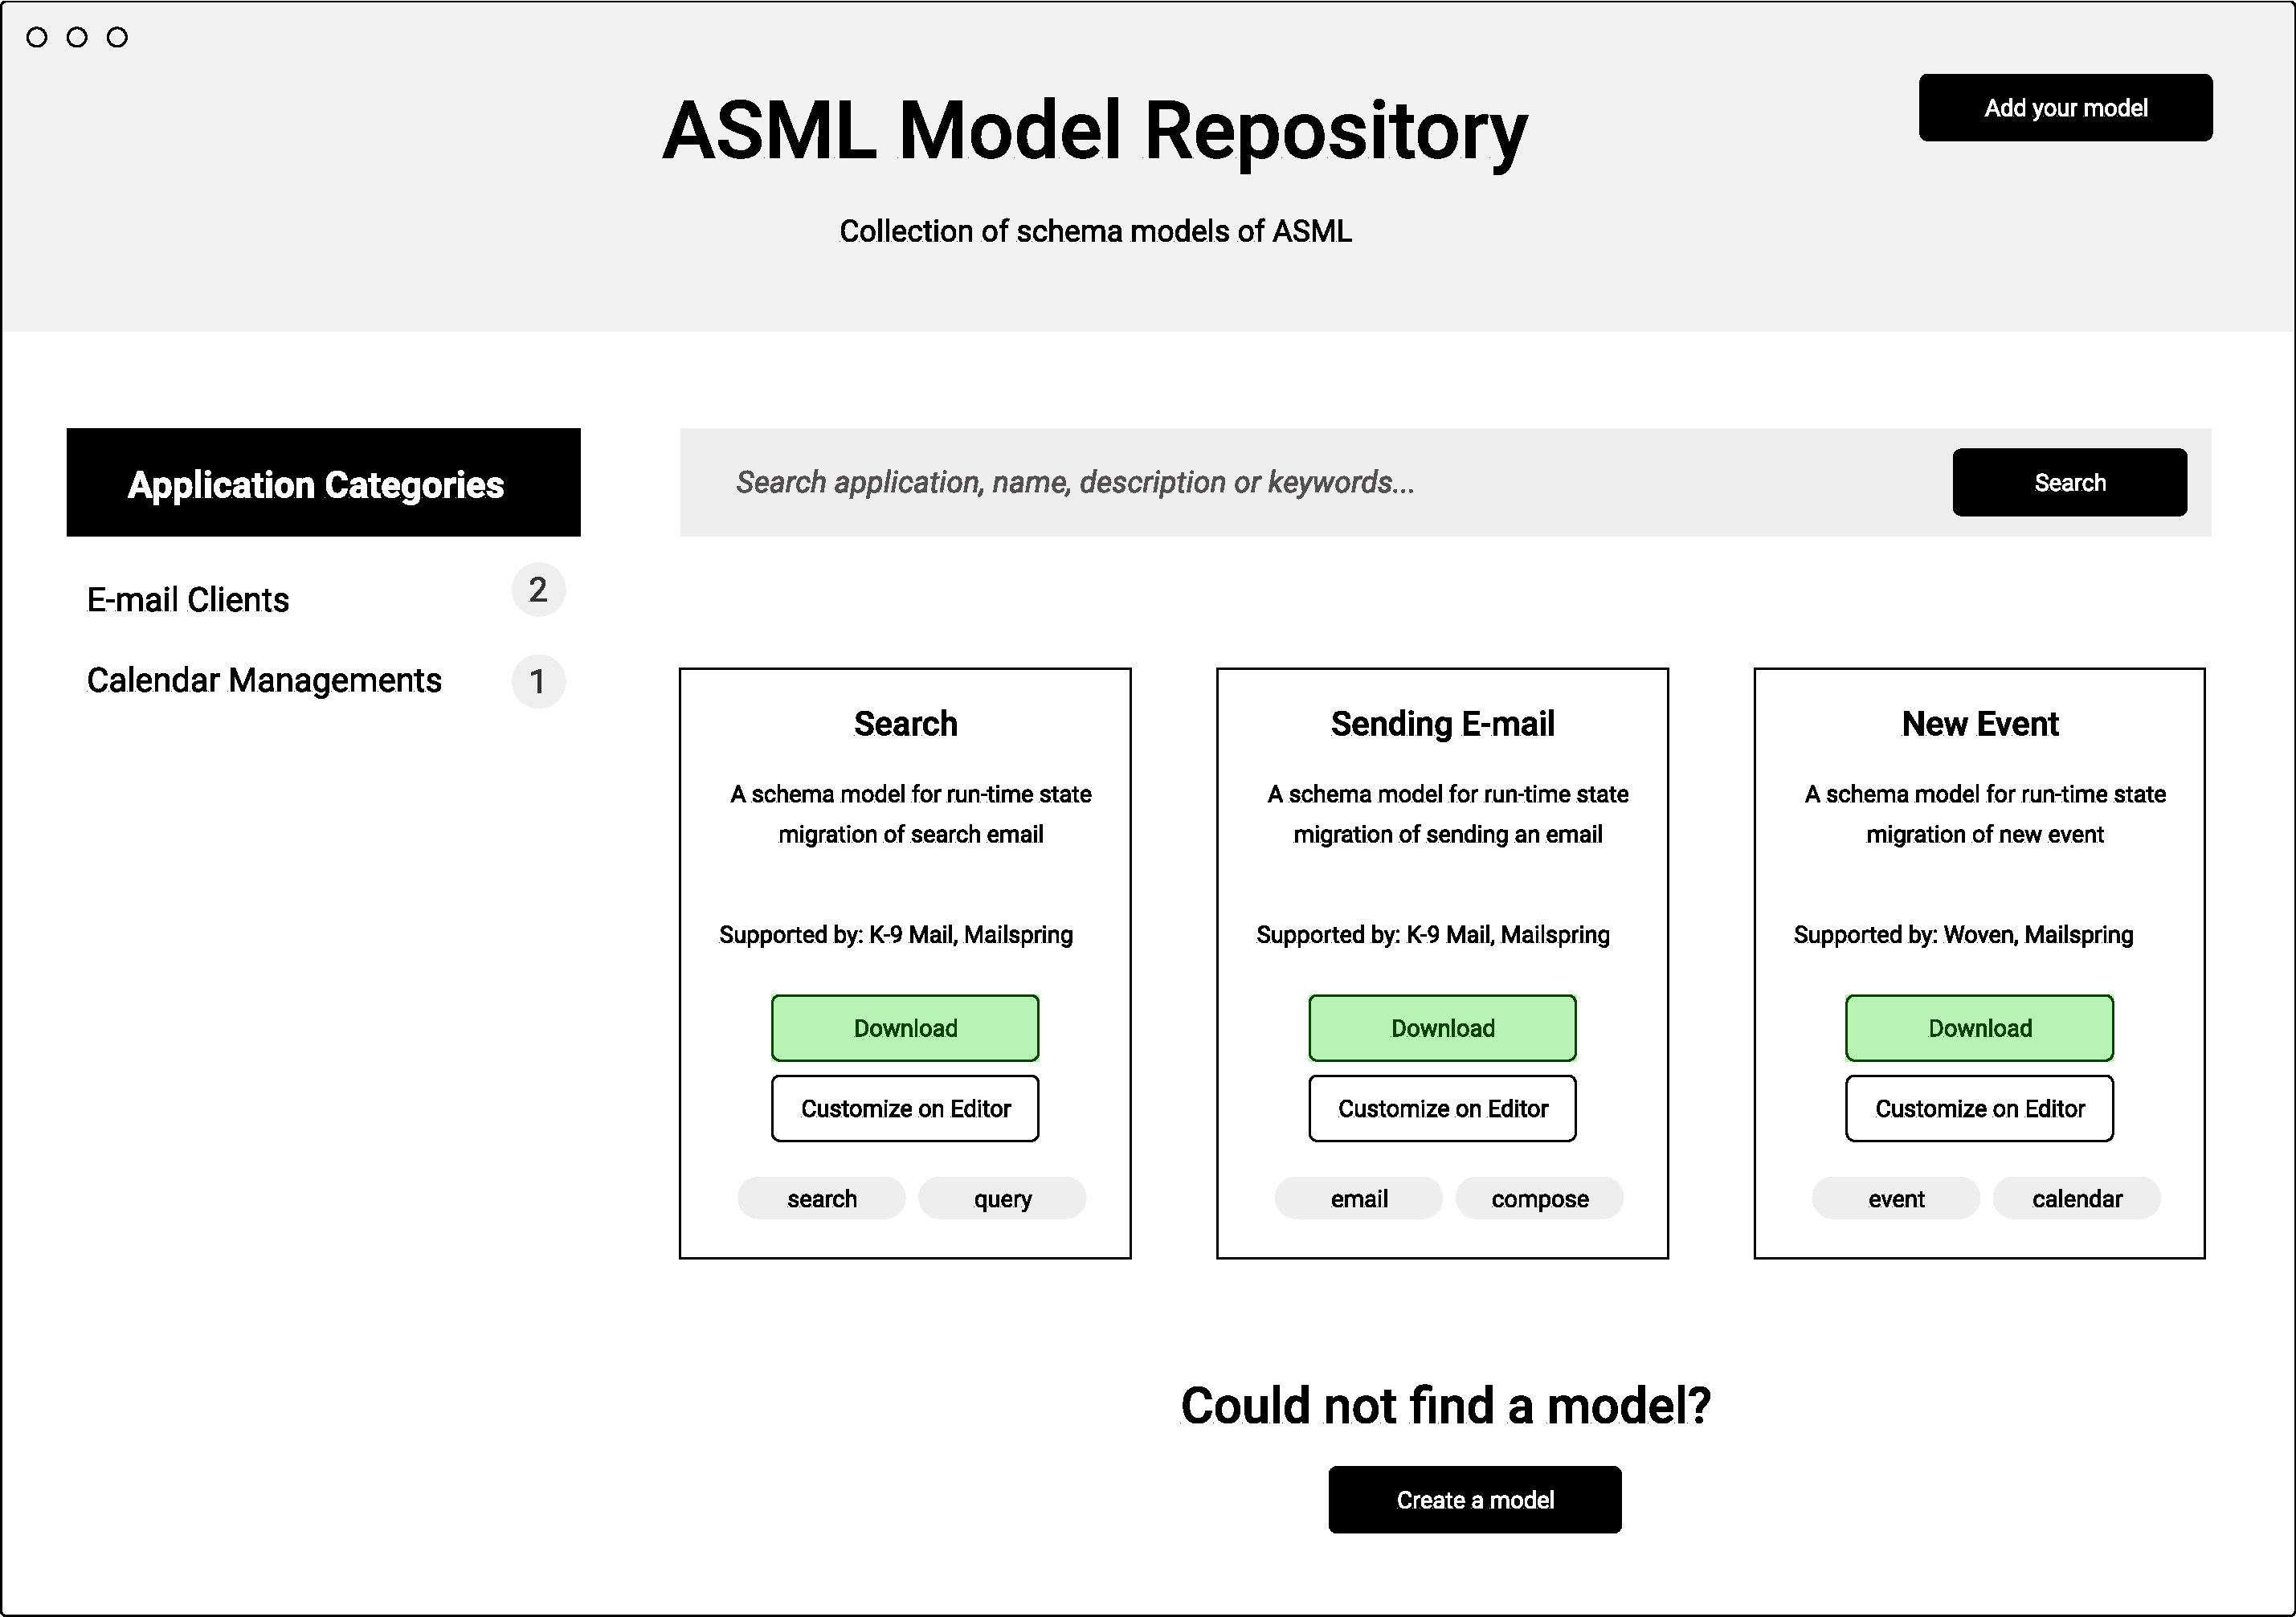
\includegraphics[width=\linewidth]{../figures/model-repo.pdf}
    \centering
    \caption{A wireframe concept for Model Repository}
    \label{fig:model-repo}
\end{figure}
\FloatBarrier